\subsection{Versuchsaufbau}
\label{sub:setup:faraday}

\begin{figure}[H]
\begin{center}
  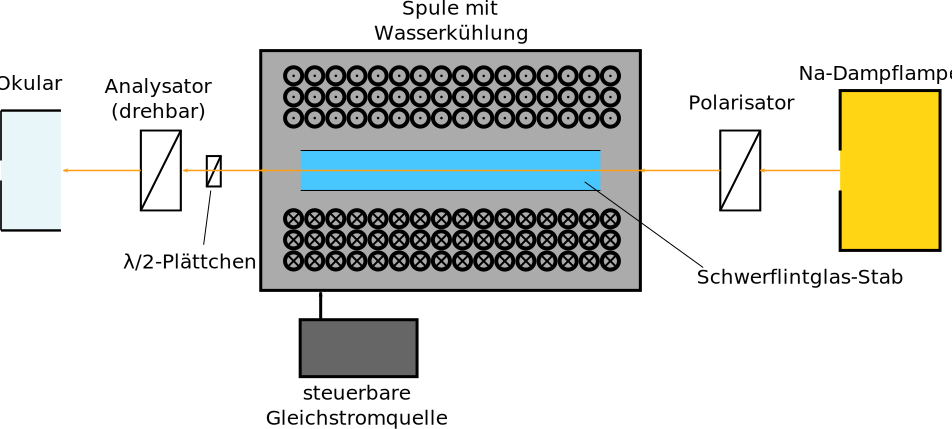
\includegraphics[width=\textwidth]{../img/aufbauFara.pdf}
  \caption{Aufbau zur Messung der Polarisationsdrehung von linear polarisiertem Licht 
  in einem Schwerflintglas-Stab im Magnetfeld einer Spule.}
  \label{img:aufbauFara}
\end{center}
\end{figure}

\autoref{img:aufbauFara} zeigt den Aufbau, der zur Messung des Faraday-Effekts verwendet wird.
Eine Natriumdampflampe liefert monochromatisches Licht ($\lambda_{\text{Na}}\approx$ 589\,nm),
das mit einem Polarisator linear polarisiert wird.
Das polarisierte Licht durchläuft dann einen Stab aus Schwerflintglas,
der sich in einer Spule befindet.
Die Spule ist wassergekühlt und wird durch ein steuerbares Netzteil mit Strom versorgt.
Nach dem Schwerflintglas wird die Polarisationsrichtung eines Teils der Strahlung von einem
\textlambda/2-Plättchen um einen kleinen Winkel gedreht.
Danach fällt der ganze Strahl durch einen drehbaren Analysator.
Diese Konfiguration wird als Halbschattenpolarimeter bezeichnet:
Wenn durch Drehung des Analysators die beiden Teile des Strahls auf gleiche Helligkeit gebracht werden,
zeigt eine Skala den Winkel, um den das Licht im Polarimeter in seiner Polarisation gedreht wird.


